\section*{Теория}

\subsection*{Основные положения волновой теории света}

Электромагнитная волна согласно уравнениям Максвелла описывается уравнением:
\begin{equation}
\nabla^2 E - \frac{1}{v^2} \frac{\partial^2 E}{\partial t^2} = 0
\label{eq:wave_gen}
\end{equation}
где $v = \frac{c}{n}$ -- скорость распространения электромагнитной волны в 
среде.

Волна называется монохроматической, если она описывается уравнением 
гармонических колебаний и её спектр состоит из одной гармоники на частоте 
$\omega$. Плоская монохроматическая волна описывается уравнением:
$$
E(\boldsymbol{r}, t) = a \cos \left( \omega t - \boldsymbol{k} \cdot 
\boldsymbol{r} \right)
$$

Сферической волной называется волна, которая описывается уравнением:
$$
E(r, t) = \frac{a}{r} \cos{\omega t - k r}
$$

Если перейти к описанию электромагнитных волн в комплексной форме:
$$
E(\boldsymbol{r}, t) = f(\boldsymbol{r}) e^{-i \omega t}
$$
и подставить полученное соотношение в уравнение (\ref{eq:wave_gen})), то 
получится уравнение Гельмгольца для комплексных амплитуд:
$$
\nabla^2 f + k^2 f = 0
$$

\subsection*{Интерференция двух монохроматических волн}

Амплитуда результирующих колебаний в точке наблюдения при интерференции 
монохроматических волн складывается по правилу суперпозиции. Тогда 
интенсивность результирующих колебаний определяется соотношением:
$$
I = I_1 + I_2 + 2 \sqrt{I_1 I_2} \cos \Delta \phi
$$
где $I_1$ и $I_2$ -- интенсивности интерферирующих волн, $\Delta \phi = \phi_1 
- \phi_2$ -- разность фаз между ними.

Если складываются волны одинаковой интенсивности $I_1 = I_2 = I_0$, то 
интерференционная картина описывается выражением:
$$
I = 2 I_0 \left( 1 + \cos \Delta \phi \right)
$$

При интерферировании волн от одного источника разность фаз определяется 
разностью проходимых лучами оптических путей $\Delta \phi = k (\Delta)$, где 
$\Delta = n_2 l_2 - n_1 l_1$ -- оптическая разность хода. Тогда результирующая 
интесивность в точке наблюдения определяется выражением:
$$
I = 2I_0 \left( 1 + \cos \frac{\omega}{c} \Delta \right)
$$

Контрастность интерференционной картины характеризуется физической величиной, 
называемой видностью $V$. По определению
$$
V = \frac{I_{max} - I_{min}}{I_{max} + I_{min}}
$$

\subsection*{Кольца Ньютона}

\begin{wrapfigure}{l}{0.3 \textwidth}
	\centering
	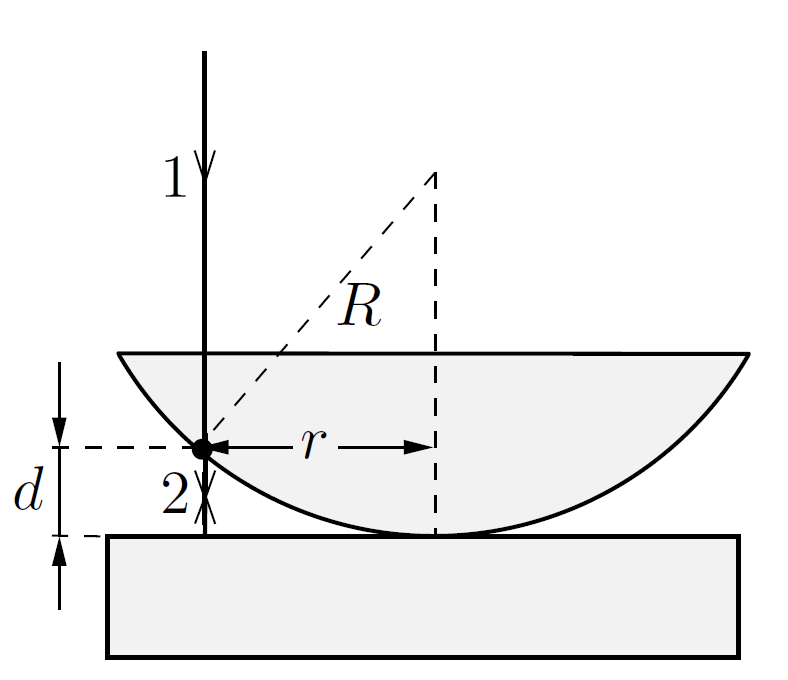
\includegraphics[width=0.28\textwidth]{../Изображения/Кольца Ньютона.png}
\end{wrapfigure}

Рассмотрим интерференционную схему колец Ньютона. Над плоской пластинкой 
размещают плосковыпуклую линзу с радиусом кривизны $R$, выпуклой стороной к 
пластинке. Свет 
распространяется от удалённого источника параллельным пучком перпендикулярно 
плоской поверхности линзы. Первый луч преломляется на сферической поверхности 
линзы, отражается от пластинки и затем отражается от линзы. Второй луч 
преломляется на сферической поверхности линзы  и интерферирует с первым лучом 
на пластинке. В приближении малой кривизны поверхности линзы можно пренебречь 
отклонением лучей от перпендикулярного распространения поверхности пластинки. 
Тогда разность фаз складывается из двойного прохождения первым 
лучом воздушной прослойки между пластинкой и линзой толщиной $d$ и набега фазы 
$\pi$ при отражении от линзы -- оптически более плотной среды:
$$
\Delta = 2 d + \frac{\lambda}{2} = \frac{r^2}{R} + \frac{\lambda}{2}
$$

Условие наблюдения интерференционного минимума задаётся выражением:
$$
\Delta = m \lambda + \frac{\lambda}{2}
$$
где $m = 0, 1, 2, \dots$.

Радиусы тёмных колец вычисляются по формуле:
$$
r_m = \sqrt{m \lambda R}
$$
Радиусы светлых колец определяются выражением:
$$
r_m' = \sqrt{(m - \frac{1}{2}) \lambda R}
$$